\begin{frame}{Contexto Histórico - La barrera clásica (1873)}
\textbf{Ernst Abbe} demostró que la resolución depende de la difracción, no solo de la calidad de las lentes.

\vspace{0.6em}
\[
  d = \frac{\lambda}{2n\sin\alpha} = \frac{\lambda}{2NA}
\]

\begin{itemize}
  \item Para luz visible, el límite práctico es \(\sim 200\,\text{nm}\).
  \item Virus, proteínas y ultraestructura celular quedan fuera del alcance óptico.
  \item Abbe anticipó la salida: usar radiación con \(\lambda\) mucho menor.
\end{itemize}
\end{frame}

\begin{frame}{Contexto Historico - Antecedentes}
\begin{columns}[T,totalwidth=\textwidth]
\column{0.49\textwidth}
\textbf{Comportamiento ondulatorio de la materia}

\vspace{0.4em}
De Broglie (1924):
\[
\lambda = \frac{h}{p}
\]

Para electrones acelerados por un potencial \(V\):
\[
\lambda \approx \frac{h}{\sqrt{2m_e eV}}
\]

\begin{itemize}
  \item A \(100\,\text{kV}\), \(\lambda_e \approx 0.0037\,\text{nm}\).
  \item \(\lambda_e\) es más de \(10^5\) veces menor que la luz visible.
\end{itemize}

\column{0.49\textwidth}
\textbf{Trabajo de Hans Busch (1926)}

\vspace{0.4em}
Busch propuso que los \textbf{campos magnéticos} podían dirigir haces de electrones de forma análoga a las lentes ópticas.

\begin{itemize}
  \item Demostró que un haz de pequeño ángulo puede enfocarse en un punto con una lente magnética cilíndrica.
  \item Esta prueba fundó la óptica electrónica práctica.
  \item Fue la base directa del desarrollo del TEM.
\end{itemize}
\end{columns}
\end{frame}

\begin{frame}{Contexto Histórico - Nacimiento del TEM (1931--1933)}





En Berlín, \textbf{Max Knoll} y \textbf{Ernst Ruska} materializaron la óptica electrónica.

\begin{itemize}
  \item Base teórica: Hans Busch (1926), lentes magnéticas axials.
  \item 1931: primer prototipo funcional de microscopio electrónico.
  \item 1933: versión que supera la resolución de la microscopía óptica.
\end{itemize}

\vspace{0.6em}
\textbf{Controversia de patente:}
\begin{itemize}
  \item Siemens registró patente en 1931 antes de la presentación pública.
  \item El reconocimiento científico recayó en Ruska.
  \item Nobel de Física en 1986 por su contribución decisiva.
\end{itemize}
\end{frame}

\begin{frame}{Contexto Histórico - Impacto}
\begin{columns}[c,totalwidth=\textwidth]
\column{0.53\textwidth}
\textbf{Impacto científico}
\begin{itemize}
  \item Descubrimiento de ribosomas (Palade, 1955).
  \item Cartografía de retículo endoplásmico, Golgi, lisosomas y mitocondrias.
  \item Nobel de 1974 (Claude, Palade y de Duve).
\end{itemize}

\column{0.46\textwidth}
\begin{figure}
  \centering
  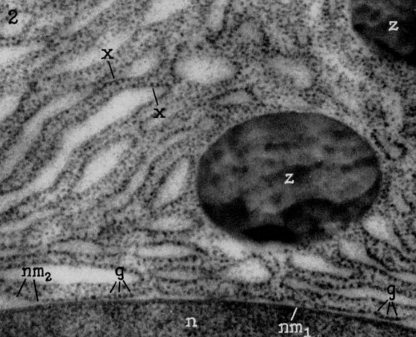
\includegraphics[width=\linewidth]{Screenshot_20260317_232844.png}
  \caption{Micrografía electrónica del retículo endoplásmico de células acinares pancreáticas de rata.}
\end{figure}
\end{columns}
\end{frame}